\chapter{Cuerpos y volúmenes}\label{ch:g9:solids}

La geometría del espacio empieza con una pequeña familia de cuerpos --- \omterm{def:g7:areas:prism}{prismas},
\omterm{def:g7:areas:prism}{cilindros}, \omterm{def:g8:solids:def}{pirámides}, \omterm{def:g8:solids:def}{conos}, esferas --- y dos preguntas: ¿cuánto
caben (\omterm{def:g6:measure:volume}{volumen}) y qué se ve al cortarlos (secciones)?
El capítulo se cierra con un hecho de gran importancia práctica: escalar un
cuerpo con factor $k$ multiplica su \omterm{def:g6:measure:volume}{volumen} por $k^3$.

\section{Los cuerpos clásicos y sus volúmenes}

\begin{theorem}[Fórmulas de volumen]\label{thm:g9:solids:volumes}
Escribe $B$ para el \omterm{def:g6:measure:area}{área} de la base y $h$ para la altura (la distancia
entre la base y la cara o el \omterm{def:g5:solids:def}{vértice} opuestos).
\begin{center}
\renewcommand{\arraystretch}{1.5}
\begin{tabular}{l|l}
cuerpo & \omterm{def:g6:measure:volume}{volumen} \\
\hline
\omterm{def:g7:areas:prism}{prisma}, \omterm{def:g7:areas:prism}{cilindro} & $V = B \times h$ \\[5pt]
\omterm{def:g8:solids:def}{pirámide}, \omterm{def:g8:solids:def}{cono} & $V = \dfrac13\, B \times h$ \\[5pt]
esfera de \omterm{def:g3:shapes:shapes}{radio} $r$ & $V = \dfrac43\,\pi r^3$ \\
\end{tabular}
\end{center}
Para un \omterm{def:g7:areas:prism}{cilindro} y un \omterm{def:g8:solids:def}{cono} de \omterm{def:g3:shapes:shapes}{radio} $r$, el \omterm{def:g6:measure:area}{área} de la base es $B = \pi r^2$;
el \omterm{def:g6:measure:area}{área} de la superficie de la esfera es $4\pi r^2$.
\end{theorem}
\admitted

\begin{omfigure}
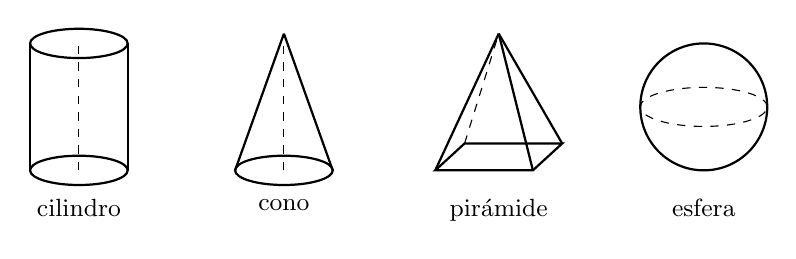
\begin{tikzpicture}[scale=0.62]
  % cilindro
  \draw[thick] (0,0) ellipse (1 and 0.3);
  \draw[thick] (-1,0) -- (-1,2.6);
  \draw[thick] (1,0) -- (1,2.6);
  \draw[thick] (0,2.6) ellipse (1 and 0.3);
  \draw[dashed] (0,0) -- (0,2.6);
  \node[below, font=\small] at (0,-0.4) {cilindro};
  % cono
  \begin{scope}[xshift=4.2cm]
  \draw[thick] (0,0) ellipse (1 and 0.3);
  \draw[thick] (-1,0) -- (0,2.8);
  \draw[thick] (1,0) -- (0,2.8);
  \draw[dashed] (0,0) -- (0,2.8);
  \node[below, font=\small] at (0,-0.4) {cono};
  \end{scope}
  % piramide
  \begin{scope}[xshift=8.4cm]
  \draw[thick] (-1.1,0) -- (0.9,0) -- (1.5,0.55) -- (-0.5,0.55) -- cycle;
  \draw[thick] (-1.1,0) -- (0.2,2.8);
  \draw[thick] (0.9,0) -- (0.2,2.8);
  \draw[thick] (1.5,0.55) -- (0.2,2.8);
  \draw[dashed] (-0.5,0.55) -- (0.2,2.8);
  \node[below, font=\small] at (0.2,-0.4) {pirámide};
  \end{scope}
  % esfera
  \begin{scope}[xshift=12.8cm]
  \draw[thick] (0,1.3) circle (1.3);
  \draw[dashed] (0,1.3) ellipse (1.3 and 0.4);
  \node[below, font=\small] at (0,-0.4) {esfera};
  \end{scope}
\end{tikzpicture}

{\small Los cuerpos de este capítulo. En cada uno, el \omterm{def:g6:measure:volume}{volumen} usa un \omterm{def:g6:measure:area}{área}
de base y una altura --- salvo la esfera, a la que solo le hace falta su \omterm{def:g3:shapes:shapes}{radio}.}
\end{omfigure}

\begin{example}\label{ex:g9:solids:volumes}
Un bote cilíndrico tiene \omterm{def:g3:shapes:shapes}{radio} $4$ cm y altura $10$ cm:
\[
V = \pi r^2 h = \pi \times 16 \times 10 = 160\pi \approx 503 \text{ cm}^3
\approx 0.5 \text{ L}.
\]
Un \omterm{def:g8:solids:def}{cono} con la misma base y la misma altura contiene un tercio de eso:
$\frac{160\pi}{3} \approx 168$ cm$^3$. Una esfera de \omterm{def:g3:shapes:shapes}{radio} $4$ cm:
$V = \frac43 \pi \times 64 = \frac{256\pi}{3} \approx 268$ cm$^3$.
\end{example}

\begin{example}[Una pirámide paso a paso]\label{ex:g9:solids:pyramid}
Una \omterm{def:g8:solids:def}{pirámide} tiene base cuadrada de lado $6$ m y altura $5$ m.
\begin{enumerate}
  \item \omterm{def:g6:measure:area}{área} de la base: $B = 6^2 = 36$ m$^2$;
  \item \omterm{def:g6:measure:volume}{volumen}: $V = \frac13 \times 36 \times 5 = 60$ m$^3$.
\end{enumerate}
Cuidado con las unidades: si el lado viniera en cm y la altura en m, habría que
convertir una de las dos primero.
\end{example}

\section{Secciones por planos}

\begin{proposition}[Secciones de los cuerpos clásicos]\label{prop:g9:solids:sections}
Cortar un cuerpo con un plano produce una figura plana, su
\emph{sección}\index{sección}:
\begin{itemize}
  \item un \omterm{def:g7:areas:prism}{prisma} o un \omterm{def:g7:areas:prism}{cilindro} cortados \emph{paralelamente a su base} dan una copia
        de la base, a cualquier altura;
  \item una \omterm{def:g8:solids:def}{pirámide} o un \omterm{def:g8:solids:def}{cono} cortados paralelamente a su base dan una
        \emph{reducción} de la base: a distancia $d$ del \omterm{def:g5:solids:def}{vértice},
        el \omterm{def:g9:thales:scaling}{factor de escala} es $k = \frac{d}{h}$;
  \item una esfera de \omterm{def:g3:shapes:shapes}{radio} $r$ cortada por un plano a distancia $d < r$ del
        centro da una circunferencia de \omterm{def:g3:shapes:shapes}{radio} $\sqrt{r^2 - d^2}$ (por el
        teorema de Pitágoras).
\end{itemize}
\end{proposition}
\admitted

\begin{omfigure}
\begin{tikzpicture}[scale=0.75]
  % cono con seccion
  \draw[thick] (0,0) ellipse (1.5 and 0.45);
  \draw[thick] (-1.5,0) -- (0,4.0);
  \draw[thick] (1.5,0) -- (0,4.0);
  \draw[omThm, thick, fill=omThm!12] (0,2.4) ellipse (0.6 and 0.18);
  \draw[dashed] (0,0) -- (0,4.0);
  \node[right, font=\small] at (0.1,4.0) {vértice};
  \draw[Stealth-Stealth, thin] (2.1,0) -- (2.1,4.0);
  \node[right, font=\small] at (2.1,2.0) {$h$};
  \draw[Stealth-Stealth, thin, omThm] (0.9,2.4) -- (0.9,4.0);
  \node[right, font=\small, omThm] at (0.92,3.2) {$d$};
  % esfera con seccion
  \begin{scope}[xshift=7.6cm]
  \draw[thick] (0,2) circle (1.8);
  \draw[omThm, thick, fill=omThm!12] (0,2.9) ellipse (1.56 and 0.4);
  \fill (0,2) circle (1.5pt) node[below, font=\small] {$O$};
  \draw[thin] (0,2) -- (0,2.9) node[midway, left, font=\small] {$d$};
  \draw[thin] (0,2.9) -- (1.56,2.9)
    node[midway, above, font=\small] {$\sqrt{r^2 - d^2}$};
  \draw[thin] (0,2) -- (-1.27,0.72)
    node[midway, below right=-3pt, font=\small] {$r$};
  \end{scope}
\end{tikzpicture}

{\small Izquierda: cortar un \omterm{def:g8:solids:def}{cono} paralelamente a su base a distancia $d$ del
\omterm{def:g5:solids:def}{vértice} da un disco escalado con $k = \frac dh$. Derecha: un plano a
distancia $d$ del centro de una esfera la corta en una circunferencia de \omterm{def:g3:shapes:shapes}{radio}
$\sqrt{r^2 - d^2}$.}
\end{omfigure}

\begin{example}\label{ex:g9:solids:section}
Un \omterm{def:g8:solids:def}{cono} tiene \omterm{def:g3:shapes:shapes}{radio} de la base $6$ y altura $9$. La \omterm{prop:g9:solids:sections}{sección} por un plano
paralelo a la base, a distancia $3$ del \omterm{def:g5:solids:def}{vértice}, es un disco escalado con
$k = \frac39 = \frac13$: su \omterm{def:g3:shapes:shapes}{radio} es $6 \times \frac13 = 2$.

Una esfera de \omterm{def:g3:shapes:shapes}{radio} $5$ se corta por un plano a distancia $3$ de su
centro: la \omterm{prop:g9:solids:sections}{sección} es una circunferencia de \omterm{def:g3:shapes:shapes}{radio} $\sqrt{25 - 9} = 4$.
\end{example}

\section{Escalar cuerpos}

\begin{theorem}[Efecto de un escalado sobre longitudes, áreas y volúmenes]\label{thm:g9:solids:scaling}
Cuando un cuerpo se amplía o se reduce con el \omterm{def:g9:thales:scaling}{factor de escala} $k > 0$:
\begin{itemize}
  \item todas las longitudes quedan multiplicadas por $k$;
  \item todas las \omterm{def:g6:measure:area}{áreas} quedan multiplicadas por $k^2$;
  \item todos los volúmenes quedan multiplicados por $k^3$.
\end{itemize}
\end{theorem}
\admitted

\begin{example}\label{ex:g9:solids:scaling}
Un coche a escala $\frac{1}{18}$: las longitudes son las del coche real
multiplicadas por $k = \frac{1}{18}$, la superficie pintada queda multiplicada por
$k^2 = \frac{1}{324}$ y el \omterm{def:g6:measure:volume}{volumen} por $k^3 = \frac{1}{5832}$.

Duplicar el \omterm{def:g3:shapes:shapes}{radio} de una esfera ($k = 2$) multiplica su \omterm{def:g6:measure:volume}{volumen} por
$2^3 = 8$: compruébalo en la fórmula,
$\frac43\pi (2r)^3 = \frac43 \pi \times 8r^3$.
\end{example}

\begin{example}[Tronco de cono]\label{ex:g9:solids:truncated}
Un \omterm{def:g8:solids:def}{cono} de altura $9$ y \omterm{def:g3:shapes:shapes}{radio} de la base $6$ (\omterm{def:g6:measure:volume}{volumen}
$\frac13 \pi \times 36 \times 9 = 108\pi$) se corta a distancia $3$ del
\omterm{def:g5:solids:def}{vértice} y se quita el \omterm{def:g8:solids:def}{cono} pequeño de encima del corte. El \omterm{def:g8:solids:def}{cono} pequeño es
la reducción con $k = \frac13$, así que su \omterm{def:g6:measure:volume}{volumen} es
$108\pi \times \left(\frac13\right)^3 = 4\pi$. El cuerpo que queda (un
\emph{tronco de \omterm{def:g8:solids:def}{cono}}) tiene \omterm{def:g6:measure:volume}{volumen} $108\pi - 4\pi = 104\pi \approx 327$.
\end{example}

\section{Ejercicios}

\begin{exercise}[$\star$]\label{exo:g9:solids:1}
Calcula los volúmenes: un \omterm{def:g5:solids:def}{ortoedro} (\omterm{def:g7:areas:prism}{prisma} rectangular) de dimensiones $4 \times 5
\times 12$; un \omterm{def:g7:areas:prism}{cilindro} de \omterm{def:g3:shapes:shapes}{radio} $3$ y altura $7$ (valor exacto con
$\pi$ y después redondeado a la unidad).
\end{exercise}

\begin{exercise}[$\star$]\label{exo:g9:solids:2}
Calcula el \omterm{def:g6:measure:volume}{volumen} de un \omterm{def:g8:solids:def}{cono} de \omterm{def:g3:shapes:shapes}{radio} $5$ y altura $12$, y el de una
\omterm{def:g8:solids:def}{pirámide} de base rectangular $8 \times 3$ y altura $10$.
\end{exercise}

\begin{exercise}[$\star$]\label{exo:g9:solids:3}
Calcula el \omterm{def:g6:measure:volume}{volumen} y el \omterm{def:g6:measure:area}{área} de la superficie de una esfera de \omterm{def:g3:shapes:shapes}{radio} $6$ (valores
exactos con $\pi$).
\end{exercise}

\begin{exercise}[$\star$]\label{exo:g9:solids:4}
Una esfera de \omterm{def:g3:shapes:shapes}{radio} $10$ se corta por un plano a distancia $8$ de su
centro. ¿Cuál es el \omterm{def:g3:shapes:shapes}{radio} de la circunferencia de la \omterm{prop:g9:solids:sections}{sección}?
\end{exercise}

\begin{exercise}[$\star\star$]\label{exo:g9:solids:5}
Un \omterm{def:g8:solids:def}{cono} tiene \omterm{def:g3:shapes:shapes}{radio} de la base $8$ y altura $12$. Un plano paralelo a la base
lo corta a distancia $9$ del \omterm{def:g5:solids:def}{vértice}. Calcula el \omterm{def:g3:shapes:shapes}{radio} de la
\omterm{prop:g9:solids:sections}{sección} y después el \omterm{def:g6:measure:volume}{volumen} del \omterm{def:g8:solids:def}{cono} pequeño de encima del corte.
\end{exercise}

\begin{exercise}[$\star\star$]\label{exo:g9:solids:6}
Un vaso cilíndrico de \omterm{def:g3:shapes:shapes}{radio} interior $3$ cm contiene agua hasta una altura de
$10$ cm. Se sumerge del todo en él una bola de \omterm{def:g3:shapes:shapes}{radio} $2$ cm. ¿Cuánto
sube el nivel del agua? (El \omterm{def:g6:measure:volume}{volumen} añadido se reparte sobre el \omterm{def:g6:measure:area}{área} de la
base del vaso; da la subida exacta y después redondea al milímetro.)
\end{exercise}

\begin{exercise}[$\star\star$]\label{exo:g9:solids:7}
Una receta llena un molde esférico de \omterm{def:g3:shapes:shapes}{radio} $6$ cm. Solo tienes un
molde esférico de \omterm{def:g3:shapes:shapes}{radio} $3$ cm. ¿Cuántos moldes pequeños puedes llenar?
(Responde sin calcular explícitamente ninguno de los dos volúmenes.)
\end{exercise}

\begin{exercise}[$\star\star$]\label{exo:g9:solids:8}
La Gran \omterm{def:g8:solids:def}{Pirámide} de Guiza tiene base cuadrada de lado unos $230$ m y una
altura de unos $147$ m. Estima su \omterm{def:g6:measure:volume}{volumen} y exprésalo en millones
de metros cúbicos.
\end{exercise}

\begin{exercise}[$\star\star\star$]\label{exo:g9:solids:9}
Un embudo con forma de \omterm{def:g8:solids:def}{cono} de \omterm{def:g3:shapes:shapes}{radio} $6$ cm y altura $12$ cm, con el \omterm{def:g5:solids:def}{vértice} hacia abajo, se
llena de agua hasta la \omterm{def:g3:division:half}{mitad} de su \emph{altura} (medida desde el
\omterm{def:g5:solids:def}{vértice}).
\begin{enumerate}
  \item ¿qué \omterm{def:g9:fractions:fraction}{fracción} del \omterm{def:g6:measure:volume}{volumen} del embudo está llena?;
  \item si, en cambio, se llena con la \omterm{def:g3:division:half}{mitad} de su \emph{\omterm{def:g6:measure:volume}{volumen}} de agua,
        demuestra que la altura $d$ del agua cumple
        $\left(\frac{d}{12}\right)^3 = \frac12$, y da $d$ al
        milímetro ($\sqrt[3]{0.5} \approx 0.7937$).
\end{enumerate}
\end{exercise}

\section{Problema: La lápida de Arquímedes}

\begin{problem}[{Problema de fin de semana --- la esfera es dos tercios de
su cilindro (por partida doble), la pila 1:2:3 y la ley del cuadrado-cubo
que prohíbe los gigantes}]
\label{pb:g9:solids:1}
Arquímedes demostró muchos teoremas, pero uno le enorgulleció tanto que
pidió que se grabara su \emph{figura} en su tumba: una esfera
encajada en su \omterm{def:g7:areas:prism}{cilindro} más ajustado. Un siglo después, el escritor romano
Cicerón, buscando entre las zarzas cerca de Siracusa, reconoció la
tumba «por la esfera y el \omterm{def:g7:areas:prism}{cilindro}». Este problema recupera
lo que el grabado codifica --- un doble milagro de dos tercios --- y después
sigue los volúmenes y las superficies (\cref{thm:g9:solids:volumes},
\cref{thm:g9:solids:scaling}) hasta una ley que gobierna a los gigantes, a las hormigas
y a los planetas que se enfrían.

\medskip
\noindent\textbf{Parte I --- El grabado descifrado.}
Una esfera de \omterm{def:g3:shapes:shapes}{radio} $r$ está encajada exactamente dentro de un \omterm{def:g7:areas:prism}{cilindro}: mismo
\omterm{def:g3:shapes:shapes}{radio}, altura $2r$.
\begin{enumerate}
  \item calcula el \omterm{def:g6:measure:volume}{volumen} del \omterm{def:g7:areas:prism}{cilindro} en función de $r$;
  \item calcula la razón entre el \omterm{def:g6:measure:volume}{volumen} de la esfera y el del
        \omterm{def:g7:areas:prism}{cilindro}. ¿Por qué le pudo gustar a Arquímedes que la
        respuesta no contenga ni $\pi$ ni $r$?;
  \item ahora las superficies: compara el \omterm{def:g6:measure:area}{área} de la superficie de la esfera con
        la superficie \emph{total} del \omterm{def:g7:areas:prism}{cilindro} (la parte lateral más
        las dos tapas). ¿Qué razón aparece --- otra vez?;
  \item el espacio vacío entre la esfera y el \omterm{def:g7:areas:prism}{cilindro} tiene \omterm{def:g6:measure:volume}{volumen}
        $2\pi r^3 - \frac43\pi r^3$. Demuestra que ese sobrante
        es exactamente igual al \omterm{def:g6:measure:volume}{volumen} de \emph{dos \omterm{def:g8:solids:def}{conos}} de \omterm{def:g3:shapes:shapes}{radio}
        $r$ y altura $r$;
  \item un balón de baloncesto de \omterm{def:g3:shapes:shapes}{radio} $12$ cm se vende en la caja
        cilíndrica más ajustada. Calcula los dos volúmenes (redondeando a
        $100$ cm$^3$) y el porcentaje de la caja que queda
        vacío.
\end{enumerate}

\medskip
\noindent\textbf{Parte II --- Cuencos, moldes y lunas.}
\begin{enumerate}[resume]
  \item un cuenco semiesférico tiene \omterm{def:g3:shapes:shapes}{radio} $10$ cm. Calcula su
        \omterm{def:g2:measure:units}{capacidad}, en cm$^3$ y en litros (al decilitro);
  \item la pila 1:2:3: un \omterm{def:g8:solids:def}{cono}, una semiesfera y un \omterm{def:g7:areas:prism}{cilindro},
        todos de \omterm{def:g3:shapes:shapes}{radio} $10$ cm y altura $10$ cm. Calcula los
        tres volúmenes y verifica la legendaria proporción
        $1 : 2 : 3$. (Esta también le habría gustado a
        Arquímedes.);
  \item una esfera de chocolate de \omterm{def:g3:shapes:shapes}{radio} $3$ cm se funde en un
        molde cilíndrico de \omterm{def:g3:shapes:shapes}{radio} $3$ cm. ¿Qué altura alcanza el
        chocolate? (\omterm{def:g9:fractions:fraction}{Fracción} exacta y después al
        milímetro.);
  \item el \omterm{def:g3:shapes:shapes}{radio} de la Tierra es de unos $6\,371$ km y el de la Luna,
        de unos $1\,737$ km. Calcula la razón de los \omterm{def:g3:shapes:shapes}{radios} y después
        --- con el \cref{thm:g9:solids:scaling} --- la razón de
        los volúmenes: ¿cuántas Lunas cabrían en una Tierra
        hueca, en \omterm{def:g6:measure:volume}{volumen}?;
  \item del mismo teorema: ¿cuál es la razón Tierra--Luna de las
        \emph{\omterm{def:g6:measure:area}{áreas} de superficie}? Y, en general, cuando el
        \omterm{def:g3:shapes:shapes}{radio} de un globo se duplica, ¿qué le pasa a su \omterm{def:g6:measure:volume}{volumen} y a su
        superficie? Enuncia la \emph{ley del cuadrado-cubo}: cuando una forma
        se escala hacia arriba, los volúmenes adelantan a las superficies.
\end{enumerate}

\medskip
\noindent\textbf{Parte III --- La ley del cuadrado-cubo gobierna el
mundo.}
\begin{enumerate}[resume]
  \item el argumento de Galileo contra los gigantes: imagina un ser humano
        escalado con un factor $10$, con las mismas proporciones. ¿Por qué
        factor crece el peso (el peso sigue al \omterm{def:g6:measure:volume}{volumen})? ¿Por qué
        factor crece la \omterm{prop:g9:solids:sections}{sección} de los huesos
        (un \omterm{def:g6:measure:area}{área})? ¿Por qué factor crece entonces la \emph{presión}
        sobre cada centímetro cuadrado de hueso --- y qué le
        pasa al gigante?;
  \item la misma ley al revés explica las hazañas de las hormigas: la fuerza
        sigue a la \omterm{prop:g9:solids:sections}{sección} del músculo (un \omterm{def:g6:measure:area}{área}) y el peso sigue al
        \omterm{def:g6:measure:volume}{volumen}. Para un animal $100$ veces más pequeño en todas las
        direcciones, ¿por qué factores se encogen el peso y la fuerza,
        y por qué factor mejora la razón entre fuerza
        y peso?;
  \item el calor lo produce el \omterm{def:g6:measure:volume}{volumen} del cuerpo y se pierde por
        su superficie. Demuestra que, para una esfera, la
        razón superficie-volumen es $\frac{3}{r}$, y calcúlala
        para $r = 1$ y $r = 2$. ¿Quién se enfría antes, un ratón o
        un oso --- y por qué los bebés necesitan gorro en invierno?;
  \item dos naranjas esféricas de \omterm{def:g3:shapes:shapes}{radios} $4$ cm y $5$ cm se
        venden al mismo precio. Calcula la razón de sus
        volúmenes: ¿cuánta más naranja da la grande por
        el mismo dinero?;
  \item final: describe con precisión qué codifica la figura de la lápida
        --- los dos «dos tercios» de las preguntas 2 y 3
        --- y responde a Cicerón en una frase: ¿por qué elegiría un
        matemático, por encima de todas las conquistas de su
        genio ingenieril, una esfera dentro de un \omterm{def:g7:areas:prism}{cilindro}?
\end{enumerate}
\end{problem}
